\def\xxactivite{Cours}

\def\xxauteur{P. Bessonnat -- Xavier Pessoles}
\fichefalse \proftrue \tdfalse \courstrue

\def\xxnumchapitre{Chapitre 11 \vspace{.2cm}}

\def\xxchapitre{Introduction aux graphes}

\def\xxcompetences{%
\textsl{%
\textbf{Savoirs et compétences :}\\
\begin{itemize}[label=\ding{112},font=\color{bleuxp}] 
\item Vocabulaire des graphes : graphe orienté, graphe non orienté. Sommet (ou nœud); arc, arête. Boucle. Degré (entrant et sortant). Chemin d’un sommet à un autre. Cycle. Connexité dans les graphes non orientés.
\item Notations : graphe $G=(S,A)$, degrés $d(s)$ (pour un graphe non orienté), $d_{+}(s)$ et  $d_{-}(s)$ (pour un graphe orienté).
\item Pondération d’un graphe. Étiquettes des arcs ou des arêtes d’un graphe. On motive l’ajout d’information à un graphe par des exemples
concrets.
\end{itemize}
}}

\def\xxfigures{
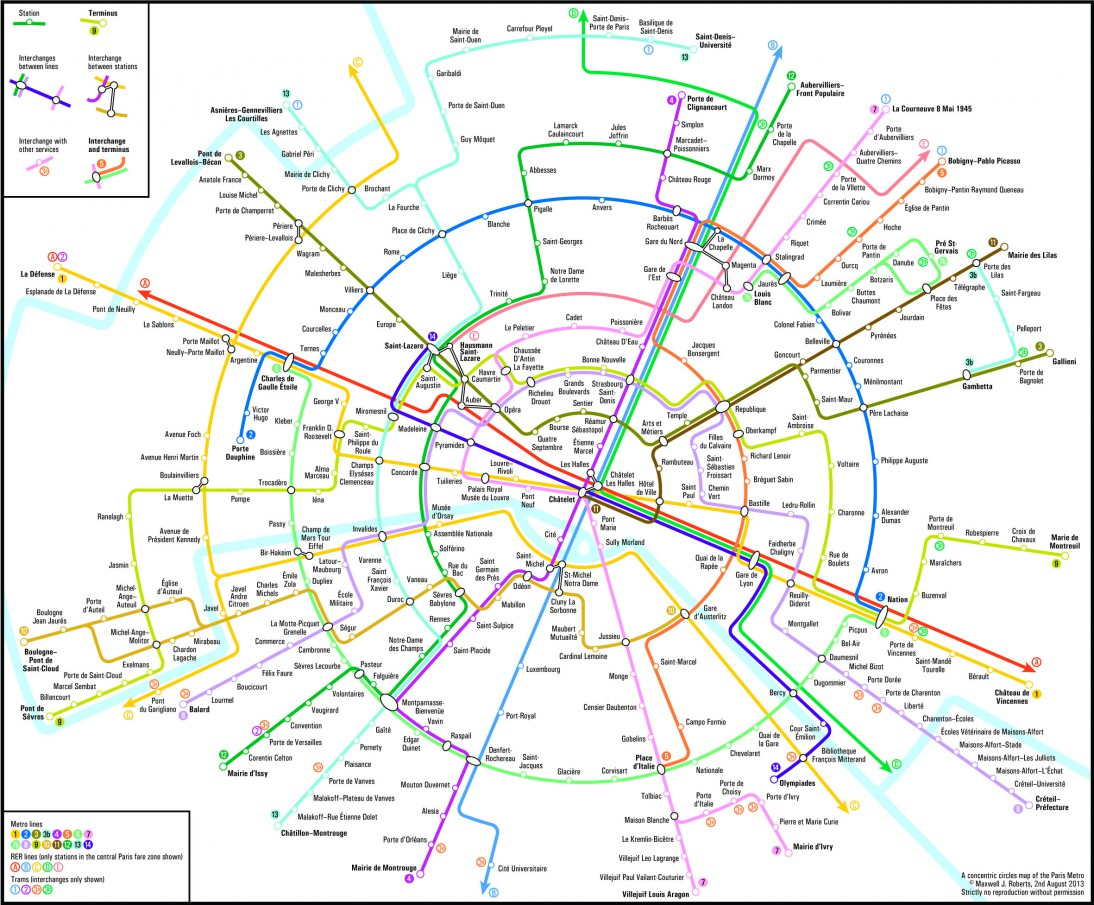
\includegraphics[width=4cm]{fig_0} \\
\textit{Représentation ciculaire du métro parisien}
}%figues de la page de garde


\input{\repRel/Style/pagegarde_cours_minitoc}
\setlength{\columnseprule}{.1pt}

\vspace{2cm}
\pagestyle{fancy}
\thispagestyle{plain}

%Thème : Tris.

\section{Compléments sur le chapitre précédent}

\subsection{Taille d'un graphe}

\begin{defi}{Taille d'un graphe}
Soit un graphe $G=\left(V,E\right)$ composé de sommets $V$ et d'arêtes $E$. On appelle taille du graphe la quantité $|V|+|E|$.
\end{defi}

\begin{rem}
On retrouve dans des ouvrages la notation $|V|$ ou $|E|$ correpondant respectivement au nombre de sommets et d'arêtes. 
Ainsi, si un algorithme est linéaire en la taille du graphe, on pourra utilisé la notation $\mathcal{O}\left(|V|+|E|\right)$.
\end{rem}

\subsection{Formule des degrés}
\begin{defi}{Formule des degrés}
Soit un graphe $G=\left(V,E\right)$, alors : $\displaystyle{\Sigma_{v \in V}} \text{deg}(v) = 2|E|$.
\end{defi}

\subsection{Graphe complet}

\begin{defi}{Graphe complet}
Un graphe complet est un graphe possédant toutes les arêtes possibles. 
\end{defi}

\begin{rem}
\begin{itemize}
\item Le nombre maximal d'arêtes d'un graphe à $n$ sommets est donné par : $\begin{pmatrix} n \\ 2\end{pmatrix}$.
\item Pour chaque sommet $v$ on a $d\degres (v) = n-1$.
\item Le nombre d'arêtes est en $\mathcal{O}\left(|V|^2\right)$.
\end{itemize}
\end{rem}

\subsection{Matrices d'adjacences}

\begin{minipage}[t]{.47\linewidth}
\begin{center}
\textbf{Avantages}
\end{center}
\begin{itemize}
\item Le test d’adjacence de deux sommets se fait en temps constant.
\item Dans le cas d’un graphe orienté, obtenir les prédécesseurs n’est pas plus compliqué (ni plus coûteux)
que d’obtenir les successeurs.
\item Rajouter ou supprimer une arête (ou un arc) peut se faire en temps constant.
%\item Il est possible de n’utiliser qu’un bit par coefficient de la matrice : dans le cas d’un graphe dense,
%une telle représentation est donc très compacte.
\end{itemize}
\end{minipage}
\hfill
\begin{minipage}[t]{.47\linewidth}
\begin{center}
\textbf{Inconvénients}
\begin{itemize}
\item Ajouter ou supprimer un sommet nécessite un temps proportionnel à $n^2$.
\item Pour récupérer les voisins/successeurs d’un noeud, il faut parcourir toute la ligne de la matrice :
l’opération se fait donc en$\mathcal{O}(n)$\footnote{$\Theta(n)$}, ce qui est regrettable si le degré sortant du noeud est petit devant $n$.
\item On consomme une mémoire proportionnelle à $|V|^2$, même quand la taille du graphe est de l’ordre de $n$ (graphe creux).
\end{itemize}
\end{center}
\end{minipage}

\subsection{Listes d'adjacences}

\begin{minipage}[t]{.47\linewidth}
\begin{center}
\textbf{Avantages}
\end{center}
\begin{itemize}
\item La mémoire utilisée est de l’ordre de $|E| + |V|$, ce qui est nettement mieux que $|V|^2$ si le graphe est
creux.
\item On a directement accès à la liste des voisins d’un noeud : la parcourir prend un temps proportionnel
au degré sortant du noeud.% (et pas à $|V|$).
\item Ajouter un noeud peut normalement se faire en temps $|V|$ (si l’ajout n’impose pas de renuméroter
les noeuds déjà présents).
\end{itemize}
\end{minipage}
\hfill
\begin{minipage}[t]{.47\linewidth}
\begin{center}
\textbf{Inconvénients}
\begin{itemize}
%\item  Si l’on a besoin d’un accès en temps raisonnable aux prédécesseurs d’un noeud (dans le cas orienté),
%il faut stocker séparément le tableau de listes correspondant.
\item Le test d’adjacence ne se fait plus en temps constant (mais en temps proportionnel au degré du
noeud).
\item Si le graphe est dense, on consommera plus de mémoire (d’un facteur constant) qu’avec une matrice
d’adjacence.
\item Ajouter ou supprimer une arête n’est pas aussi évident que dans une matrice d’adjacence : suivant
l’opération précise que l’on souhaite faire, la complexité peut être unitaire ou proportionnelle aux
degrés des noeuds impactés.
\item  Supprimer un noeud n’est pas pratique : le plus simple est de reconstruire entièrement le graphe (en
un temps $\mathcal{O}\left(|E| + |V|\right)$).
\end{itemize}
\end{center}
\end{minipage}

\section{Parcours de graphe}
Une fois que nous sommes en présence d'un graphe, il va falloir le parcourir pour répondre à différentes questions : 
\begin{itemize}
\item est-il possible de joindre un sommet $A$ et un sommet $B$ ?
\item est-il possible, depuis un sommet, de rejoindre tous les autres sommets du graphe ?
\item peut-on détecter la présence de cycle ou de circuit dans un graphe ?
\item quel est le plus court chemin pour joindre deux sommets ?
\item \textit{etc.}
\end{itemize}

Les deux algorithmes principaux sont les suivants :
\begin{itemize}
\item le parcours en largeur -- \textit{Breadth-First Search} (BFS) -- pour lequel on va commencer par visiter les sommets les plus proches du sommet initial (sommets de niveau 1), puis les plus proches des sommets de niveau 1 \textit{etc.};
\item le parcours en profondeur  -- \textit{Depth-First Search} (DFS) -- pour lequel on part d'un sommet initial jusqu'au sommet le plus loin. On remonte alors la pile pour explorer les ramifications.
\end{itemize}

Une des difficultés du parcours de graphe est d'éviter de tourner en rond. C'est pour cela qu'on mémorisera l'information d'avoir visité ou non un sommet. 

\subsection{Parcours en largeur}

\subsubsection{Un premier algorithme}
On propose ci-dessous un algorithme de parcours en largeur en utilisant un graphe implémenté sous forme de liste d'adjacence ainsi qu'un sommet \texttt{s} de départ. 

\begin{lstlisting}
def bfs(G:dict, s:str) -> None:
    """
    G : graphe sous forme de dictionnaire d'adjacence
    s : sommet du graphe (Chaine de caractere du type "S1").
    """
    visited = {}
    for sommet,voisins in G.items():
        visited[sommet] = False
    # Le premier sommet à visiter entre dans la file
    file = deque([s])
    while len(file) > 0:
        # On visite la tête de file
        tete = file.pop()
        # On vérifier qu'elle n'a pas été visitée
        if not visited[tete]:
            # Si on l'avait pas visité, maintenant c'est le cas :)
            visited[tete] = True            
            # On met les voisins de tete dans la file
            for v in G[tete]:
                file.appendleft(v)
\end{lstlisting}

Dans cet algorithme : 
\begin{itemize}
\item on commence par créer une liste ayant pour taille le nombre de sommets. Cette liste va permettre de savoir si un sommet a été visité ou non;
\item dans la file, on va commencer par ajouter le sommet initial;
\item on commence alors à traiter la file en extrayant l'indice du sommet initial;
\item si ce sommet n'a pas été visité, il devient visité;
\item on ajoute alors dans la file l'ensemble des voisins du sommet initial;
\item on continue alors de traiter la file. 
\end{itemize}

\begin{rem}
En l'état, à quoi sert cet algorithme ?
\end{rem}


\subsubsection{Applications}
\begin{exemple}
\textit{Comment connaître la distance d'un sommet \texttt{s} aux autres?}
\ifprof
\begin{lstlisting}
def distances(G, s):
    dist = [-1]*len(G)
    q = deque([(s, 0)])
    while len(q) > 0:
        u, d = q.pop()
        if dist[u] == -1:
            dist[u] = d
            for v in G[u]:
                q.appendleft((v, d + 1))
    return dist
\end{lstlisting}
\else
\vspace{5cm}
\fi
\end{exemple}

\begin{exemple}
\textit{Comment connaître un plus court chemin d’un sommet s à un autre ? }
\ifprof
\begin{lstlisting}
def bfs(G, s):
    pred = [-1]*len(G)
    q = deque([(s, s)])
    while len(q) > 0:
        u, p = q.pop()
        if pred[u] == -1:
            pred[u] = p
            for v in G[u]:
                q.appendleft((v, u))
    return pred
    
def path(pred, s, v):
    L = []
    while v != s:
        L.append(v)
        v = pred[v]
    L.append(s)
    return L[::-1] # inverse le chemin
\end{lstlisting}
\else
\vspace{10cm}
\fi
\end{exemple}

\subsubsection{Marquage de sommet}

\subsection{Parcours en profondeur}
\subsubsection{Un premier algorithme}

On propose ci-dessous un algorithme de parcours en profondeur en utilisant un graphe implémenté sous forme de liste d'adjacence ainsi qu'un sommet \texttt{s} de départ. 

\begin{lstlisting}
def dfs(G, s): #
    visited = [False]*len(G)
    pile = [s]
    while len(pile) > 0:
        u = pile.pop()
        if not visited[u]:
            visited[u] = True
            for v in G[u]:
                pile.append(v)
\end{lstlisting}

Dans cet algorithme : 
\begin{itemize}
\item on commence par créer une liste ayant pour taile le nombre de sommets. Cette liste va permettre de savoir si un sommet a été visité ou non;
\item dans la pile, on va commencer par ajouter le sommet initial;
\item on commence alors à traiter le sommet initial après l'avoir extrait de la pile;
\item si ce sommet n'a pas été visité, il devient visité;
\item on ajoute alors dans la pile l'ensemble des voisins du sommet initial;
\item on continue alors de traiter la pile. 
\end{itemize}
À la différence du parcours en largeur, lorsqu'on va traiter la pile, on va s'éloigner du sommet initial... avant d'y revenir quand toutes les voies auront été explorées. 

\subsubsection{Applications}
\begin{exemple}
\textit{Lister les sommets dans l'ordre de leur visite.}
\end{exemple}


\begin{exemple}
\textit{Comment déterminer si un graphe non orienté est connexe ?}
\end{exemple}


\begin{exemple}
\textit{Comment déterminer si un graphe non orienté contient un cycle ?}
\end{exemple}

\section*{Références}

\begin{itemize}
\item Cours de Quentin Fortier \url{https://fortierq.github.io/itc1/}.
\item Cours de JB Bianquis. Chapitre 5 : Parcours de graphes. Lycée du Parc. Lyon.
\item Cours de T. Kovaltchouk. Graphes : parcours. Lycée polyvalent Franklin Roosevelt, Reims.
\item \url{https ://perso.liris.cnrs.fr/vincent.nivoliers/lifap6/Supports/Cours/graph_traversal.html}
\item \url{http ://mpechaud.fr/scripts/parcours/index.html}
\end{itemize}